\documentclass[compress]{beamer}
\usecolortheme{default}

\usepackage{lmodern, epstopdf, multirow, array, setspace, bbm, tcolorbox, pbox, bm, mathtools, tikz}
\usepackage[T1]{fontenc}

\setbeamertemplate{frametitle}[default][center]
\setbeamertemplate{footline}{\hfill \insertframenumber/\inserttotalframenumber\hspace*{5pt}\vspace{5pt}}
\setbeamertemplate{navigation symbols}{}

\newlength{\wideitemsep}
\setlength{\wideitemsep}{\itemsep}
\addtolength{\wideitemsep}{4pt}
\let\olditem\item
\renewcommand{\item}{\setlength{\itemsep}{\wideitemsep}\olditem}
\setlength{\leftmargini}{12pt}
\setlength{\leftmarginii}{14pt}
\setbeamertemplate{itemize/enumerate subbody begin}{\vspace{6pt}}
\setbeamertemplate{itemize item}[circle]
\setbeamertemplate{enumerate item}[circle]
\setbeamertemplate{enumerate subitem}[default]

\setbeamercolor{alerted text}{fg=blue}
\setbeamersize{text margin left=1.5em,text margin right=1.5em}

\tcbset{
    colback=white,
    colframe=black,
    coltext=black,
    coltitle=blue,
    colbacktitle=white,
    boxrule=1pt,
    titlerule=0pt,
    toptitle=4pt,
    top=2pt
}

\newenvironment{changemargin}[2]{% 
  \begin{list}{}{% 
    \setlength{\topsep}{0pt}% 
    \setlength{\leftmargin}{#1}% 
    \setlength{\rightmargin}{#2}% 
    \setlength{\listparindent}{\parindent}% 
    \setlength{\itemindent}{\parindent}% 
    \setlength{\parsep}{\parskip}% 
  }% 
  \item[]}{\end{list}}
  
\newenvironment{defn}{%
  \begin{tcolorbox}[title={Definition}]%
  }{\end{tcolorbox}}
  
\newenvironment{prop}[1]{%
  \begin{tcolorbox}[title={Proposition #1}]%
  }{\end{tcolorbox}}
  
\newcommand{\cit}[1]{{\footnotesize \textcolor[rgb]{0.5,0,0}{#1}}}

% Font size for code listings (verbatim blocks); reset with \normalsize
\newcommand{\codesize}{\fontsize{7}{8.5}\selectfont}

\newcommand{\slidesetup}[1]{%
  \title{#1}%
  \subtitle{\texorpdfstring{\vspace{0.3\baselineskip}}{} {\small This version: \today}}%
  \author[Mikkel Plagborg-Moller]{ECMA 31150, Spring 2026 \texorpdfstring{\\[0.5ex]}{} University of Chicago \texorpdfstring{\\[0.5ex]}{} Department of Economics \texorpdfstring{\\[4ex]}{} Mikkel Plagborg-Moller}%
  \date{}%
}

% \circleoverlay[options]{text}
% Draws a red circle with a text box nearby on a tikz overlay.
% Options (with defaults):
%   cx=0cm, cy=0cm      - circle center (shift from page center)
%   r=1cm               - circle radius
%   tx=0cm, ty=0cm      - text box offset from circle center
%   text anchor=east    - anchor of text node (east = text left, west = text right)
%   font=\normalsize    - font size for text
\pgfkeys{
  /circleoverlay/.cd,
  cx/.store in=\cocx, cx=0cm,
  cy/.store in=\cocy, cy=0cm,
  r/.store in=\cor, r=1cm,
  tx/.store in=\cotx, tx=0cm,
  ty/.store in=\coty, ty=0cm,
  text anchor/.store in=\cotextanchor, text anchor=east,
  font/.store in=\cofont, font=\normalsize,
}
\newcommand{\circleoverlay}[2][]{%
  \pgfkeys{/circleoverlay/.cd, cx=0cm, cy=0cm, r=1cm, tx=0cm, ty=0cm, text anchor=east, font=\normalsize, #1}%
  \pgfmathsetlengthmacro{\circlediameter}{2*\cor}%
  \node[draw=red, line width=2pt, circle, minimum size=\circlediameter, inner sep=0pt]
    (tmpcirc) at ([xshift=\cocx,yshift=\cocy]current page.center) {};%
  \node[anchor=\cotextanchor, fill=white, draw=red, text=red, inner sep=4pt, align=left, font=\cofont]
    at ([xshift=\cotx,yshift=\coty]tmpcirc.center) {#2};%
}

\DeclareMathOperator*{\argmax}{argmax}
\DeclareMathOperator*{\argmin}{argmin}
\DeclareMathOperator{\diag}{diag}
\DeclareMathOperator{\var}{Var}
\DeclareMathOperator{\cov}{Cov}
\DeclareMathOperator{\corr}{Corr}
\DeclareMathOperator{\lrv}{LRV}

\usetikzlibrary{arrows,positioning} 
\tikzset{
    %Define standard arrow tip
    >=stealth',
    % Define arrow style
    arr/.style={
           ->,
           thick,
           shorten <=2pt,
           shorten >=2pt,}
}

\slidesetup{State space models I}

\begin{document}
\frame{
\maketitle
}

\frame{
\frametitle{Plan for this slide deck}
\begin{enumerate}
\item Modeling latent variables with state space models
\item Inferring the latent variables
\item Bayesian inference on state space models
\item Application: GDP measurement
\end{enumerate}
}

\frame{
\frametitle{Models with latent variables}
\begin{itemize}
\item In many settings, we'd like to consider models with \textbf{latent} (i.e., unobserved) variables.
\item Our observed data is related to the latent variables, but with added noise.
\item \textbf{State space models} form a rich class of models with latent variables.
\item As we'll see in the next slide deck, state space models also facilitate analysis of time-varying parameters, missing data, and mixed-frequency data.
\end{itemize}
}

\frame{
\frametitle{Linear-Gaussian state space model}
\begin{itemize}
\item \textbf{Observation equation} for $n \times 1$ observed data $\bm{y}_t$:
\[\bm{y}_t = \bm{c} + \bm{G}\bm{s}_t + \bm{v}_t,\quad \bm{v}_t \overset{iid}{\sim} N(\bm{0},\bm{V}).\]
\vspace{-1.5\baselineskip}
\begin{itemize}
\item $\bm{v}_t$: measurement error.
\end{itemize}
\item \textbf{Transition equation} for $m \times 1$ latent \textbf{state} vector $\bm{s}_t$:
\[\bm{s}_t = \bm{F}\bm{s}_{t-1} + \bm{u}_t,\quad \bm{u}_t \overset{iid}{\sim} N(\bm{0},\bm{U}).\]
\vspace{-1.5\baselineskip}
\begin{itemize}
\item $\bm{u}_t$: shocks to the state vector.
\end{itemize}
\item Initial condition:
\[\bm{s}_0 \sim N(\bm{s}_{0|0},\bm{P}_{0|0}).\]
\item $\bm{s}_0$, $\lbrace \bm{u}_t \rbrace$, and $\lbrace \bm{v}_t \rbrace$ are all mutually independent.
\end{itemize}
}

\frame{
\begin{figure}
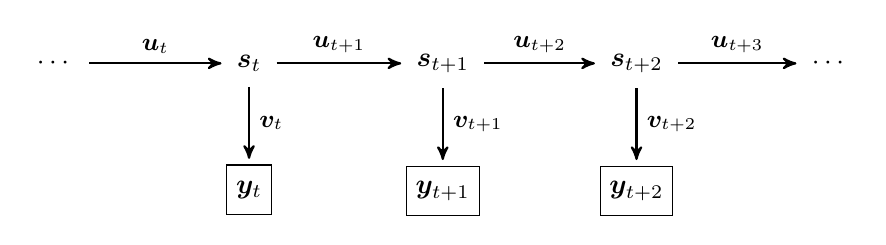
\begin{tikzpicture}[node distance=7em]
\node (ldots) {$\cdots$};
\node[right of=ldots] (St) {$\bm{s}_t$};
\node[right of=St] (Stp1) {$\bm{s}_{t+1}$};
\node[right of=Stp1] (Stp2) {$\bm{s}_{t+2}$};
\node[right of=Stp2] (rdots) {$\cdots$};

\node[draw, below=3em of St, minimum height=18pt] (Yt) {$\bm{y}_t$};
\node[draw, below=3em of Stp1, minimum height=18pt] (Ytp1) {$\bm{y}_{t+1}$};
\node[draw, below=3em of Stp2, minimum height=18pt] (Ytp2) {$\bm{y}_{t+2}$};

\draw[arr] (ldots) -- node [midway, above] {\small $\bm{u}_t$} (St);
\draw[arr] (St) -- node [midway, above] {\small $\bm{u}_{t+1}$} (Stp1);
\draw[arr] (Stp1) -- node [midway, above] {\small $\bm{u}_{t+2}$} (Stp2);
\draw[arr] (Stp2) -- node [midway, above] {\small $\bm{u}_{t+3}$} (rdots);

\draw[arr] (St) -- node [midway, right] {\small $\bm{v}_t$} (Yt);
\draw[arr] (Stp1) -- node [midway, right] {\small $\bm{v}_{t+1}$} (Ytp1);
\draw[arr] (Stp2) -- node [midway, right] {\small $\bm{v}_{t+2}$} (Ytp2);
\end{tikzpicture}
\end{figure}
}

\frame{
\frametitle{Example 1: dynamic factor model}
\begin{itemize}
\item Consider a model where $n$ observed series $y_{1t},\dots,y_{nt}$ are driven by a latent \textbf{factor} $f_t$:
\[y_{it} = c_i + \lambda_i f_t + v_{it},\quad v_{it} \overset{iid}{\sim} N(0,\sigma_i^2).\]
\item $f_t$ could be thought of as the overall state of the business cycle.
\item The idiosyncratic errors $v_{it}$ are assumed independent across $i$. So $f_t$ is responsible for the co-movement between the observed series.
\item Assume $f_t$ evolves as an AR($p$) process:
\[f_t = a_1 f_{t-1} + \dots + a_p f_{t-p} + u_t,\quad u_t \overset{iid}{\sim} N(0,1).\]
\item We need to normalize either the scale of the \textbf{loadings} $\lambda_i$ or the factor $f_t$. Here set $\var(u_t)=1$.
\end{itemize}
}

\frame{
\frametitle{Example 1: dynamic factor model (cont.)}
\begin{itemize}
\item Written in state space form:
\[\bm{y}_t = \bm{c} + \bm{G}\bm{s}_t + \bm{v}_t,\quad \bm{v}_t \overset{iid}{\sim} N(\bm{0},\bm{V}),\]
\[\bm{s}_t = \bm{F}\bm{s}_{t-1} + \bm{u}_t,\quad \bm{u}_t \overset{iid}{\sim} N(\bm{0},\bm{U}),\]
where
\[\bm{c} \equiv \begin{pmatrix}
c_1 \\
\vdots \\
c_n
\end{pmatrix},\; \bm{G} \equiv \begin{pmatrix}
\lambda_1 & 0 & \dots & 0 \\
\vdots & \vdots & \vdots & \vdots \\
\lambda_n & 0 & \dots & 0
\end{pmatrix},\; \bm{V} \equiv \begin{pmatrix}
\sigma_1^2 & & \\
 & \ddots & \\
 & & \sigma_n^2
\end{pmatrix},\]
\[\bm{s}_t \equiv \begin{pmatrix}
f_t \\
f_{t-1} \\
\vdots \\
f_{t-p+1}
\end{pmatrix},\; \bm{F} \equiv \begin{pmatrix}
a_1 & a_2 & \cdots & a_p \\
1 & & & 0 \\
 & \ddots & & \vdots \\
 & & 1 & 0
\end{pmatrix},\; \bm{U} \equiv \begin{pmatrix}
1 & & & \\
& 0 & & \\
& & \ddots & \\
& & & 0
\end{pmatrix}.\]
\end{itemize}
}

\frame{
\frametitle{Example 1: dynamic factor model (cont.)}
\begin{itemize}
\item Let's simulate data from the factor model:
\[y_{it} = c_i + \lambda_i f_t + v_{it},\quad v_{it} \overset{iid}{\sim} N(0,\sigma_i^2),\]
\[f_t = a_1 f_{t-1} + u_t,\quad u_t \overset{iid}{\sim} N(0,1).\]
\item $n=3$ observed variables $y_{1t}$, $y_{2t}$, $y_{3t}$.
\item True parameters:
\[\begin{pmatrix}
c_1 \\
c_2 \\
c_3
\end{pmatrix} = \begin{pmatrix}
1 \\
0 \\
0
\end{pmatrix},\quad \begin{pmatrix}
\lambda_1 \\
\lambda_2 \\
\lambda_3
\end{pmatrix} = \begin{pmatrix}
1 \\
-1 \\
2
\end{pmatrix},\quad \begin{pmatrix}
\sigma_1^2 \\
\sigma_2^2 \\
\sigma_3^2
\end{pmatrix} = \begin{pmatrix}
4 \\
4 \\
9
\end{pmatrix}.\]
\end{itemize}
}

\frame{
\begin{figure}
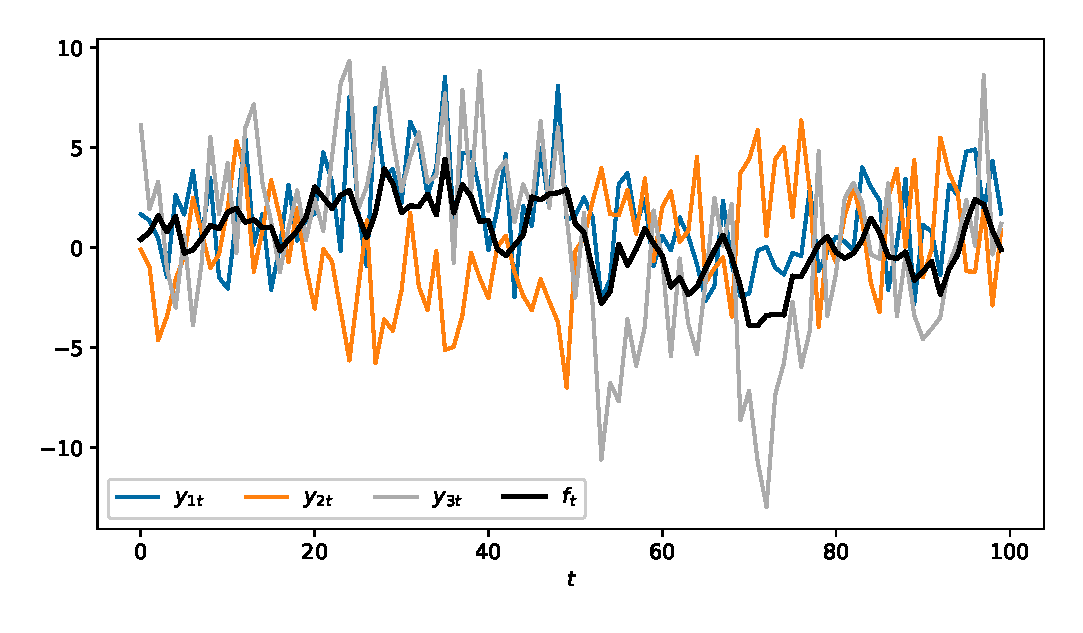
\includegraphics[width=\linewidth]{fig/factor_sim.eps}
\end{figure}
}

\frame{
\frametitle{Example 2: stationary ARMA$(1,1)$}
\[y_t = \rho y_{t-1} + u_t + \theta u_{t-1},\quad u_t \overset{iid}{\sim} N(0,\sigma^2)\]
\[\Downarrow\]
\[y_t = (1-\rho L)^{-1}(1+\theta L)u_t = (1+\theta L)x_t,\]
\[\text{where}\quad x_t \equiv (1-\rho L)^{-1}u_t \quad \text{satisfies}\quad x_t =\rho x_{t-1} + u_t\]
\[\Downarrow\]
\[y_t = \bm{G}\bm{s}_t + v_t,\quad v_t \overset{iid}{\sim} N(0,\alert{0}),\]
\[\bm{s}_t = \bm{F}\bm{s}_{t-1} + \bm{u}_t,\quad \bm{u}_t \overset{iid}{\sim} N(\bm{0},\bm{U}),\]
\[\text{where} \quad \bm{s}_t \equiv \begin{pmatrix}
x_t \\
x_{t-1}
\end{pmatrix},\; \bm{G} \equiv \begin{pmatrix}
1 & \theta
\end{pmatrix},\; \bm{F} \equiv \begin{pmatrix}
\rho & 0 \\
1 & 0
\end{pmatrix},\; \bm{U} \equiv \begin{pmatrix}
\sigma^2 & 0 \\
0 & 0
\end{pmatrix}.\]
\begin{itemize}
\item General ARMA$(p,q)$: Brockwell \& Davis textbook, Example 9.3.2.
\end{itemize}
}

\frame{
\frametitle{Inferring the latent states}
\begin{itemize}
\item How can we infer the latent states $\lbrace \bm{s}_t \rbrace$ from the observed data $\lbrace \bm{y}_t \rbrace$?
\item Assume for now that we know the true parameters of the state space model (more on estimation later).
\item Since both states and data are Gaussian, we're working with conditional distributions of Gaussian random vectors.
%\item Reminder from previous probability course:
%\[\begin{pmatrix}
%\bm{y} \\
%\bm{x}
%\end{pmatrix} \sim N\left(\begin{pmatrix}
%\bm{\mu}_y \\
%\bm{\mu}_x \\
%\end{pmatrix}, \begin{pmatrix}
%\bm{\Sigma}_y & \bm{\Sigma}_{yx} \\
%\bm{\Sigma}_{xy} & \bm{\Sigma}_x
%\end{pmatrix} \right)\]
%\[\Longrightarrow (\bm{y} \mid \bm{x}) \sim N\Big(\underbrace{\bm{\mu}_y + \bm{\Sigma}_{yx}\bm{\Sigma}_x^{-1}(\bm{x}-\bm{\mu}_x)}_{E[\bm{y} \mid \bm{x}]}, \underbrace{\bm{\Sigma}_y - \bm{\Sigma}_{yx}\bm{\Sigma}_x^{-1}\bm{\Sigma}_{xy}}_{\var(\bm{y} \mid \bm{x})}\Big).\]
\item We just need to keep track of conditional means and variances:
\[\bm{s}_{t|\tau} \equiv E[\bm{s}_t \mid \lbrace \bm{y}_s \rbrace_{1 \leq s \leq \tau}],\quad \bm{P}_{t|\tau} \equiv \var[\bm{s}_t \mid \lbrace \bm{y}_s \rbrace_{1 \leq s \leq \tau}],\]
\[\bm{y}_{t|\tau} \equiv E[\bm{y}_t \mid \lbrace \bm{y}_s \rbrace_{1 \leq s \leq \tau}],\quad \bm{Q}_{t|\tau} \equiv \var[\bm{y}_t \mid \lbrace \bm{y}_s \rbrace_{1 \leq s \leq \tau}].\]
\end{itemize}
}

\frame{
\frametitle{Inferring the latent states (cont.)}
\begin{itemize}
\item We will proceed inductively/iteratively. Take as given the information $\lbrace\bm{s}_{t-1|t-1},\bm{P}_{t-1|t-1}\rbrace$ about $\bm{s}_{t-1}$ using data up to time $t-1$.
\item Then (\alert{exercise:} verify)
\begin{align*}
\bm{s}_{t|t-1} &= E[\bm{F}\bm{s}_{t-1} + \bm{u}_t \mid \lbrace \bm{y}_s \rbrace_{s \leq t-1}] = \boxed{\bm{F}\bm{s}_{t-1|t-1}}, \\
\bm{P}_{t|t-1} &= \var(\bm{F}\bm{s}_{t-1} + \bm{u}_t \mid \lbrace \bm{y}_s \rbrace_{s \leq t-1}) = \boxed{\bm{F} \bm{P}_{t-1|t-1} \bm{F}' + \bm{U}}, \\
\bm{y}_{t|t-1} &= E[\bm{c} + \bm{G}\bm{s}_t + \bm{v}_t \mid \lbrace \bm{y}_s \rbrace_{s \leq t-1}] = \boxed{\bm{c} + \bm{G}\bm{s}_{t|t-1}}, \\
\bm{Q}_{t|t-1} &= \var(\bm{c} + \bm{G}\bm{s}_t + \bm{v}_t \mid \lbrace \bm{y}_s \rbrace_{s \leq t-1}) = \boxed{\bm{G}\bm{P}_{t|t-1}\bm{G}' + \bm{V}}.
\end{align*}
\item These formulas tell us how to forecast $\bm{s}_t$ and $\bm{y}_t$ one step ahead.
\end{itemize}
}

\frame{
\frametitle{Inferring the latent states (cont.)}
\begin{itemize}
\item $\lbrace \bm{s}_t,\bm{y}_t \rbrace$ are jointly Gaussian given $\lbrace \bm{y}_s \rbrace_{s \leq t-1}$.
\item By the standard formula for the conditional distribution of jointly Gaussian vectors (Brockwell \& Davis textbook, Proposition A.3.1):
\[\bm{s}_{t|t} = E[\bm{s}_t \mid \lbrace \bm{y}_s \rbrace_{s \leq t}] = \boxed{\bm{s}_{t|t-1} + \bm{K}_t(\bm{y}_t - \bm{y}_{t|t-1})},\]
\[\text{where}\quad \bm{K}_t \equiv \cov(\bm{s}_t,\bm{y}_t \mid \lbrace \bm{y}_s \rbrace_{s\leq t-1})\bm{Q}_{t|t-1}^{-1}.\]
\item Moreover, by that same formula,
\begin{align*}
&\bm{P}_{t|t} = \var(\bm{s}_t \mid \lbrace \bm{y}_s \rbrace_{s \leq t}) \\
&= \boxed{\bm{P}_{t|t-1} - \cov(\bm{s}_t,\bm{y}_t \mid \lbrace \bm{y}_s \rbrace_{s\leq t-1})\bm{Q}_{t|t-1}^{-1}\cov(\bm{y}_t,\bm{s}_t \mid \lbrace \bm{y}_s \rbrace_{s\leq t-1})}.
\end{align*}
\item \alert{Exercise:} use the state space model equations to show
\[\cov(\bm{s}_t,\bm{y}_t \mid \lbrace \bm{y}_s \rbrace_{s\leq t-1}) = \bm{P}_{t|t-1}\bm{G}'.\]
\end{itemize}
}

\frame{
\frametitle{Kalman filter}
\begin{itemize}
\item The preceding derivations yield the \textbf{Kalman filter} recursions:
\end{itemize}
\begin{enumerate}
\item Initialize $\lbrace \bm{s}_{0|0}, \bm{P}_{0|0}\rbrace$.
\item For each $t=1,2,\dots,T$:
\begin{enumerate}
\item[a)] \emph{Predict:}
\begin{align*}
\bm{s}_{t|t-1} &= \bm{F}\bm{s}_{t-1|t-1}, \\
\bm{P}_{t|t-1} &= \bm{F} \bm{P}_{t-1|t-1} \bm{F}' + \bm{U}, \\
\bm{y}_{t|t-1} &= \bm{c} + \bm{G}\bm{s}_{t|t-1}, \\
\bm{Q}_{t|t-1} &= \bm{G}\bm{P}_{t|t-1}\bm{G}' + \bm{V}.
\end{align*}
\item[b)] \textbf{Kalman gain}: $\bm{K}_t = \bm{P}_{t|t-1}\bm{G}' \bm{Q}_{t|t-1}^{-1}$.
\item[c)] \emph{Update:}
\begin{align*}
\bm{s}_{t|t} &= \bm{s}_{t|t-1} + \bm{K}_t(\bm{y}_t - \bm{y}_{t|t-1}), \\
\bm{P}_{t|t} &= \bm{P}_{t|t-1} - \bm{K}_t\bm{Q}_{t|t-1}\bm{K}_t'.
\end{align*}
\end{enumerate}
\end{enumerate}
}

\frame{
\frametitle{Kalman filter: initialization}
\begin{itemize}
\item We need to pick a ``prior belief'' about the initial state $\bm{s}_0$:
\[\bm{s}_0 \sim N(\bm{s}_{0|0},\bm{P}_{0|0}).\]
\item If $\lbrace \bm{s}_t \rbrace$ is stationary, it makes sense to initialize at the stationary distribution:
\[\bm{s}_{0|0} = \bm{0}, \quad \bm{P}_{0|0} = \var(\bm{s}_t),\]
where (as we know) the latter solves the Lyapunov equation
\[\var(\bm{s}_t) = \bm{F}\var(\bm{s}_t)\bm{F}' + \bm{U}.\]
\item If $\lbrace \bm{s}_t \rbrace$ is not stationary, we could choose some diffuse beliefs
\[\bm{s}_{0|0} = \bm{0}, \quad \bm{P}_{0|0} = \tau^2 \bm{I},\]
with very large $\tau^2$.
\end{itemize}
}

\begin{frame}[fragile]
\tiny
\begin{verbatim}
def kalman_filter(Y, c, G, V, F, U, s0, P0):
    T, n = Y.shape
    m = F.shape[0]

    s_pred = np.zeros((T, m))       # s_{t|t-1}
    P_pred = np.zeros((T, m, m))    # P_{t|t-1}
    s_filt = np.zeros((T, m))       # s_{t|t}
    P_filt = np.zeros((T, m, m))    # P_{t|t}
    y_pred = np.zeros((T, n))       # y_{t|t-1}
    Q_pred = np.zeros((T, n, n))    # Q_{t|t-1}

    s_prev, P_prev = s0, P0
    for t in range(T):
        # Predict
        s_pred[t] = F @ s_prev
        P_pred[t] = F @ P_prev @ F.T + U
        y_pred[t] = c + G @ s_pred[t]
        Q_pred[t] = G @ P_pred[t] @ G.T + V

        # Gain
        K = np.linalg.solve(Q_pred[t], G @ P_pred[t]).T

        # Update
        innov = Y[t] - y_pred[t]
        s_filt[t] = s_pred[t] + K @ innov
        P_filt[t] = P_pred[t] - K @ Q_pred[t] @ K.T

        s_prev, P_prev = s_filt[t], P_filt[t]

    return {'s_pred': s_pred, 'P_pred': P_pred,
            's_filt': s_filt, 'P_filt': P_filt,
            'y_pred': y_pred, 'Q_pred': Q_pred}
\end{verbatim}
\end{frame}

\frame{
\begin{figure}
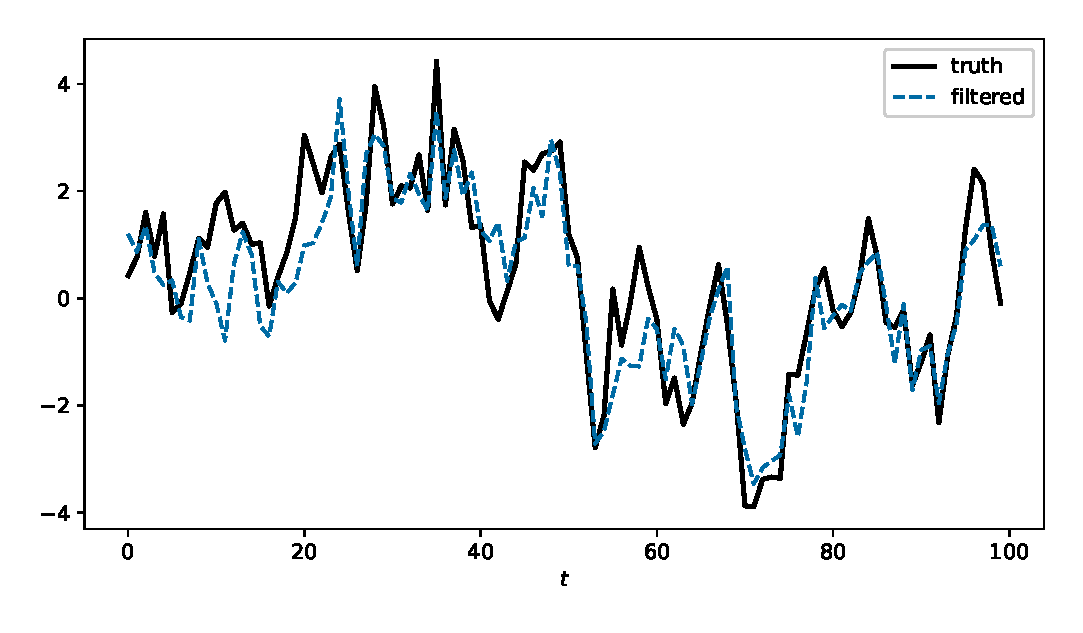
\includegraphics[width=\linewidth]{fig/factor_filter.eps} \\
\bigskip
Kalman filter applied to the simulated data from earlier
\end{figure}
}

\frame{
\frametitle{Kalman smoother}
\begin{itemize}
\item Kalman filter computes our ``posterior'' for $\bm{s}_t$ given data up to time $t$:
\[(\bm{s}_t \mid \lbrace \bm{y}_s \rbrace_{1 \leq s\leq t}) \sim N(\bm{s}_{t|t}, \bm{P}_{t|t}).\]
\item But the data \emph{after} time $t$ may also be helpful for inferring $\bm{s}_t$.
\item The \textbf{Kalman smoother} recursions (next slide) compute the full posterior:
\[(\bm{s}_t \mid \lbrace \bm{y}_s \rbrace_{1 \leq s\leq T}) \sim N(\bm{s}_{t|T}, \bm{P}_{t|T}).\]
\item Derivation: Brockwell \& Davis textbook, chapter 9.4.
\end{itemize}
}

\frame{
\frametitle{Kalman smoother: algorithm}
\begin{enumerate}
\item Run the Kalman filter to obtain $\lbrace \bm{s}_{t|t-1},\bm{P}_{t|t-1},\bm{s}_{t|t},\bm{P}_{t|t} \rbrace_{t=1}^T$.
\item For each $t=T-1,T-2,\dots,1$ (going backwards in time):
\begin{enumerate}
\item [a)] Compute $\bm{J}_t = \bm{P}_{t|t}\bm{F}'\bm{P}_{t+1|t}^{-1}$.
\item [b)] Iterate:
\end{enumerate}
\begin{align*}
\bm{s}_{t|T} &= \bm{s}_{t|t} + \bm{J}_t(\bm{s}_{t+1|T}-\bm{s}_{t+1|t}), \\
\bm{P}_{t|T} &= \bm{P}_{t|t} + \bm{J}_t(\bm{P}_{t+1|T} - \bm{P}_{t+1|t})\bm{J}_t'.
\end{align*}
\end{enumerate}
}

\begin{frame}[fragile]
\scriptsize
\begin{verbatim}
def kalman_smoother(filt, F):
    s_pred, P_pred = filt['s_pred'], filt['P_pred']
    s_filt, P_filt = filt['s_filt'], filt['P_filt']
    T, m = s_filt.shape

    s_smooth = np.zeros((T, m))     # s_{t|T}
    P_smooth = np.zeros((T, m, m))  # P_{t|T}

    # Initialize at final filtered state
    s_smooth[T - 1] = s_filt[T - 1]
    P_smooth[T - 1] = P_filt[T - 1]
    
    for t in range(T - 2, -1, -1):
        J = np.linalg.solve(P_pred[t + 1], F @ P_filt[t]).T
        s_smooth[t] = s_filt[t] + J @ (s_smooth[t + 1] - s_pred[t + 1])
        P_smooth[t] = P_filt[t] + J @ (P_smooth[t + 1] - P_pred[t + 1]) @ J.T

    return {'s_smooth': s_smooth, 'P_smooth': P_smooth}
\end{verbatim}
\bigskip
\small
Note: you can also use the pre-packaged Kalman filter and smoother in \texttt{statsmodels.tsa.statespace}. Just make sure you understand the notation.
\end{frame}

\frame{
\begin{figure}
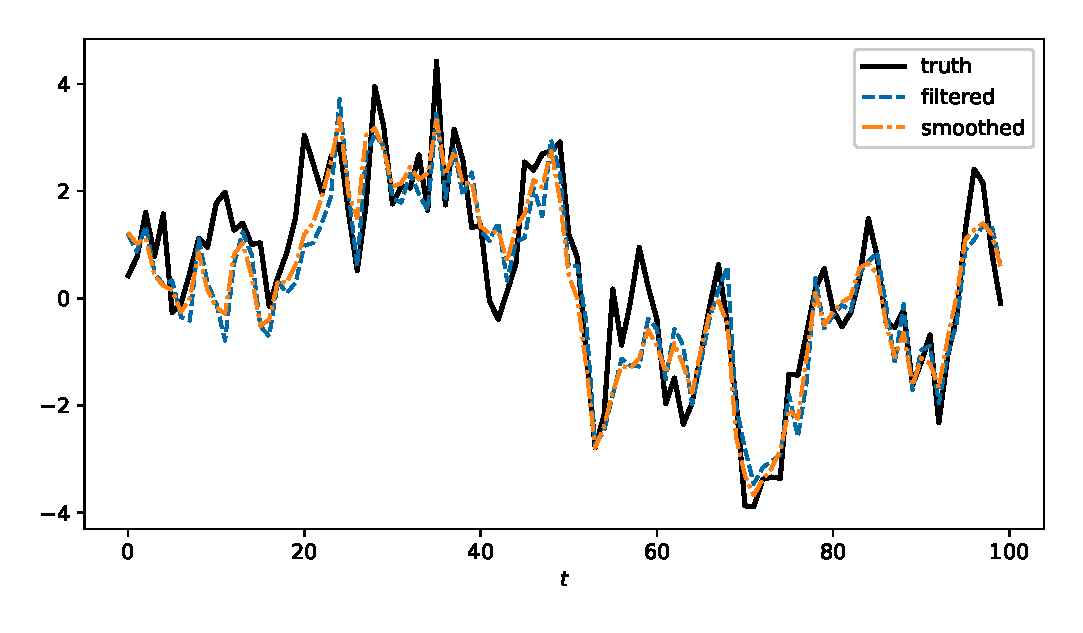
\includegraphics[width=\linewidth]{fig/factor_filter_smooth.eps} \\
\bigskip
Kalman filter and smoother applied to the simulated data from earlier
\end{figure}
}

\frame{
\begin{figure}
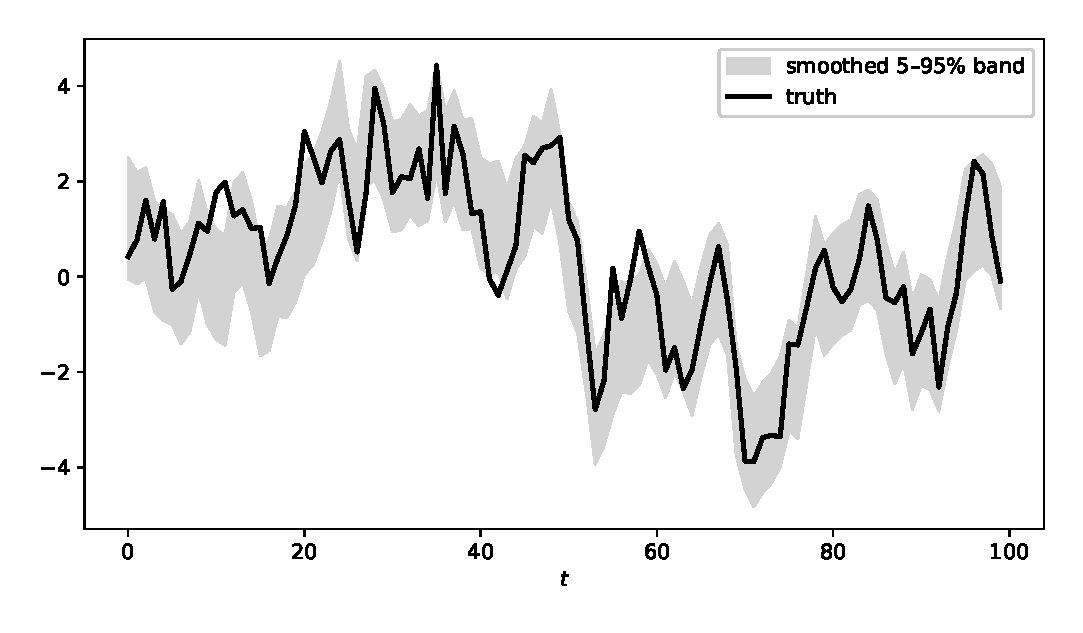
\includegraphics[width=\linewidth]{fig/factor_smooth_band.eps}
\end{figure}
}

\frame{
\frametitle{Bayesian estimation of state space models}
\begin{itemize}
\item So far we've assumed that the parameters of the state space model were known.
\item Let's now consider Bayesian estimation of these parameters.
\item Suppose we have formulated a prior on the underlying parameter vector $\bm{\theta}$. The coefficient matrices $\lbrace \bm{c},\bm{F},\bm{G},\bm{U},\bm{V} \rbrace$ are functions of $\bm{\theta}$.
\item How to compute the likelihood?
\end{itemize}
}

\frame{
\frametitle{Bayesian estimation: likelihood function}
\begin{itemize}
\item From the Kalman filter we know
\[(\bm{y}_t \mid \lbrace \bm{y}_s \rbrace_{1 \leq s\leq t-1},\bm{\theta}) \sim N(\bm{y}_{t|t-1},\bm{Q}_{t|t-1}).\]
\vspace{-1.5\baselineskip}
\begin{itemize}
\item $\bm{y}_{t|t-1}$ and $\bm{Q}_{t|t-1}$ are implicitly functions of $\bm{\theta}$.
\end{itemize}
\item This gives us all necessary ingredients for the likelihood:
\begin{align*}
&f(\bm{y}_1,\dots,\bm{y}_T \mid \bm{\theta}) = \prod_{t=1}^T f(\bm{y}_t \mid \lbrace \bm{y}_s \rbrace_{1 \leq s \leq t-1},\bm{\theta}) \\
&= \prod_{t=1}^T (2\pi)^{-n/2} \det(\bm{Q}_{t|t-1})^{-1/2}e^{-\frac{1}{2}(\bm{y}_t-\bm{y}_{t|t-1})'\bm{Q}_{t|t-1}^{-1}(\bm{y}_t-\bm{y}_{t|t-1})}.
\end{align*}
\item We could use this to compute a \textbf{maximum likelihood estimator}
\[\textstyle \hat{\bm{\theta}}^\text{MLE} \equiv \argmax_{\bm{\theta}}\, f(\bm{y}_1,\dots,\bm{y}_T \mid \bm{\theta})\]
via numerical optimization. But we will focus on Bayesian inference.
\end{itemize}
}

\frame{
\frametitle{Application: GDP measurement}
\begin{itemize}
\item The Bureau of Economic Analysis produces two measures of GDP that should theoretically be equivalent:
\begin{enumerate}
\item Expenditure-side measure $\text{GDP}_{Et}$: sum of all expenditures on final goods and services.
\item Income-side measure $\text{GDP}_{It}$: sum of all income generated in production (also called Gross Domestic Income, GDI).
\end{enumerate}
\item But in practice these two series can diverge significantly due to imperfections in data collection.
\end{itemize}
}

\frame{
\begin{figure}
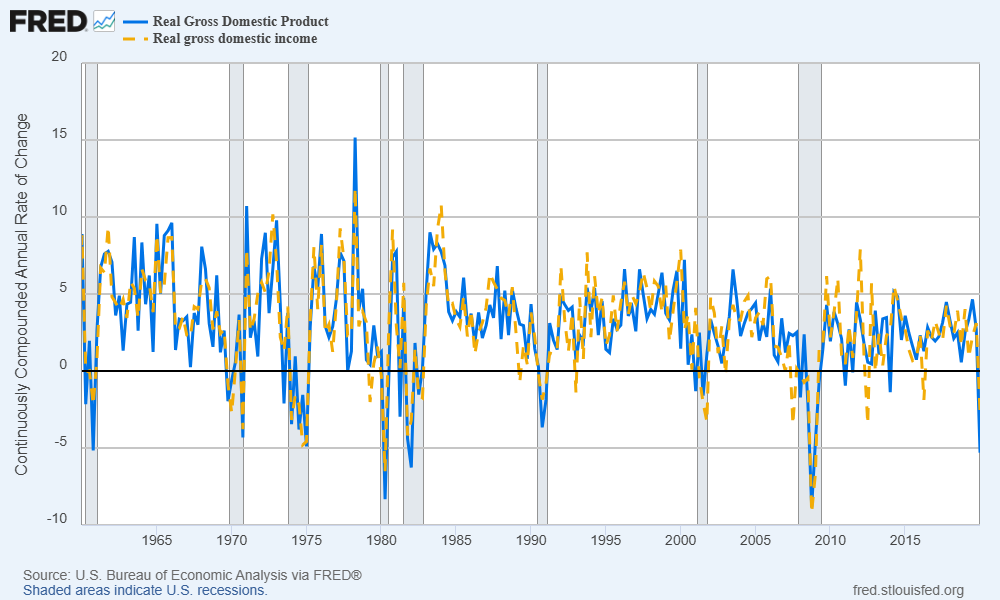
\includegraphics[width=\linewidth]{fig/fred_gdp_gdi.png}
\end{figure}
}

\begin{frame}[fragile]
\begin{verbatim}
              GDP         GDI   GDP - GDI
count  239.000000  239.000000  239.000000
mean     2.989405    2.980319    0.009085
std      3.235301    3.159994    1.953780
min     -8.853365   -9.192442   -6.430172
25%      1.397032    1.282381   -1.311526
50%      3.040811    3.235237   -0.009659
75%      4.519602    4.897933    1.228413
max     15.167842   11.874460    5.751909
\end{verbatim}
\bigskip
Units: annualized log growth rates, real
\end{frame}

\frame{
\frametitle{Application: GDP measurement (cont.)}
\begin{itemize}
\item We model the real GDP measurements as a dynamic factor model.
\begin{itemize}
\item Simplest model in Aruoba, Diebold, Nalewaik, Schorfheide \& Song (2016). See paper for more elaborate approaches.
\end{itemize}
\item Assume latent true GDP growth $\tilde{s}_t$ evolves as an AR(1):
\[\tilde{s}_t = \tilde{c} + \rho \tilde{s}_{t-1} + u_t,\quad u_t \overset{iid}{\sim} N(0,\sigma_G^2).\]
\item The two observed GDP measures are noisy proxies of true GDP:
\begin{align*}
\text{GDP}_{Et} &= \tilde{s}_t + v_{Et},\quad v_{Et} \overset{iid}{\sim} N(0,\sigma_E^2), \\
\text{GDP}_{It} &= \tilde{s}_t + v_{It},\quad v_{It} \overset{iid}{\sim} N(0,\sigma_I^2).
\end{align*}
\item Errors/shocks $\lbrace v_{Et} \rbrace$, $\lbrace v_{It} \rbrace$, and $\lbrace u_t \rbrace$ are independent of each other.
\end{itemize}
}

\frame{
\frametitle{Application: GDP measurement (cont.)}
\begin{itemize}
\item Define $s_t \equiv \tilde{s}_t - \mu$, where $\mu \equiv E[\tilde{s}_t] = \frac{\tilde{c}}{1-\rho}$.
\item State space representation:
\[\bm{y}_t = \bm{c} + \bm{G}s_t + \bm{v}_t,\quad s_t = F s_{t-1} + u_t,\]
\[\text{where}\quad \bm{y}_t \equiv \begin{pmatrix}
\text{GDP}_{Et} \\
\text{GDP}_{It}
\end{pmatrix},\quad \bm{c} \equiv \begin{pmatrix}
\mu \\
\mu
\end{pmatrix},\quad \bm{G} \equiv \begin{pmatrix}
1 \\
1
\end{pmatrix},\]
\[F \equiv \rho,\quad \var(u_t) \equiv \sigma_G^2,\quad \var(\bm{v}_t) \equiv \begin{pmatrix}
\sigma_E^2 & 0 \\
0 & \sigma_I^2
\end{pmatrix}.\]
\item Prior distribution (all parameters independent):
\[\mu \sim N(3,100),\quad \rho \sim N(0.3,1) \enskip \text{truncated to } [-1,1],\]
\[\sigma_j \sim \text{Cauchy}_+(0,5),\; j \in \lbrace E,I,G \rbrace.\]
\end{itemize}
}

\begin{frame}[fragile]
\tiny
\begin{verbatim}
data {
    int<lower=1> T;             // sample size
    matrix[T, 2] y;             // data
    real mu_mean;               // prior mean for mu
    real<lower=0> mu_std;       // prior std. dev. for mu
    real rho_mean;              // prior mean for rho
    real<lower=0> rho_std;      // prior std. dev. for rho
    real<lower=0> sigma_scale;  // prior scale for sigma_j
}

transformed data {
    vector[2] G = [1.0, 1.0]';
}

parameters {
    real mu;
    real<lower=-1, upper=1> rho;
    vector<lower=0>[2] sigma_v;
    real<lower=0> sigma_G;
}

transformed parameters {
    vector[2] c = [mu, mu]';
    matrix[2, 2] V = diag_matrix(square(sigma_v));
}
\end{verbatim}
\normalsize
(continued on next slide)
\end{frame}

\begin{frame}[fragile]
\tiny
\begin{verbatim}
model {
    // Prior
    mu ~ normal(mu_mean, mu_std);
    rho ~ normal(rho_mean, rho_std);
    sigma_v ~ cauchy(0, sigma_scale);
    sigma_G ~ cauchy(0, sigma_scale);

    // Likelihood via Kalman filter
    {
        // Initialize
        real s = 0;
        real P = square(sigma_G) / (1 - square(rho));

        for (t in 1:T) {
            // Predict
            real s_pred = rho * s;
            real P_pred = square(rho) * P + square(sigma_G);
            vector[2] y_pred = c + G * s_pred;
            matrix[2, 2] Q_pred = P_pred * G * G' + V;

            // Likelihood contribution
            y[t]' ~ multi_normal(y_pred, Q_pred);

            // Gain (transposed)
            vector[2] Kt = mdivide_left_spd(Q_pred, G * P_pred);

            // Update
            s = s_pred + Kt' * (y[t]' - y_pred);
            P = P_pred - Kt' * Q_pred * Kt;
        }
    }
}
\end{verbatim}
\end{frame}

\frame{
\begin{figure}
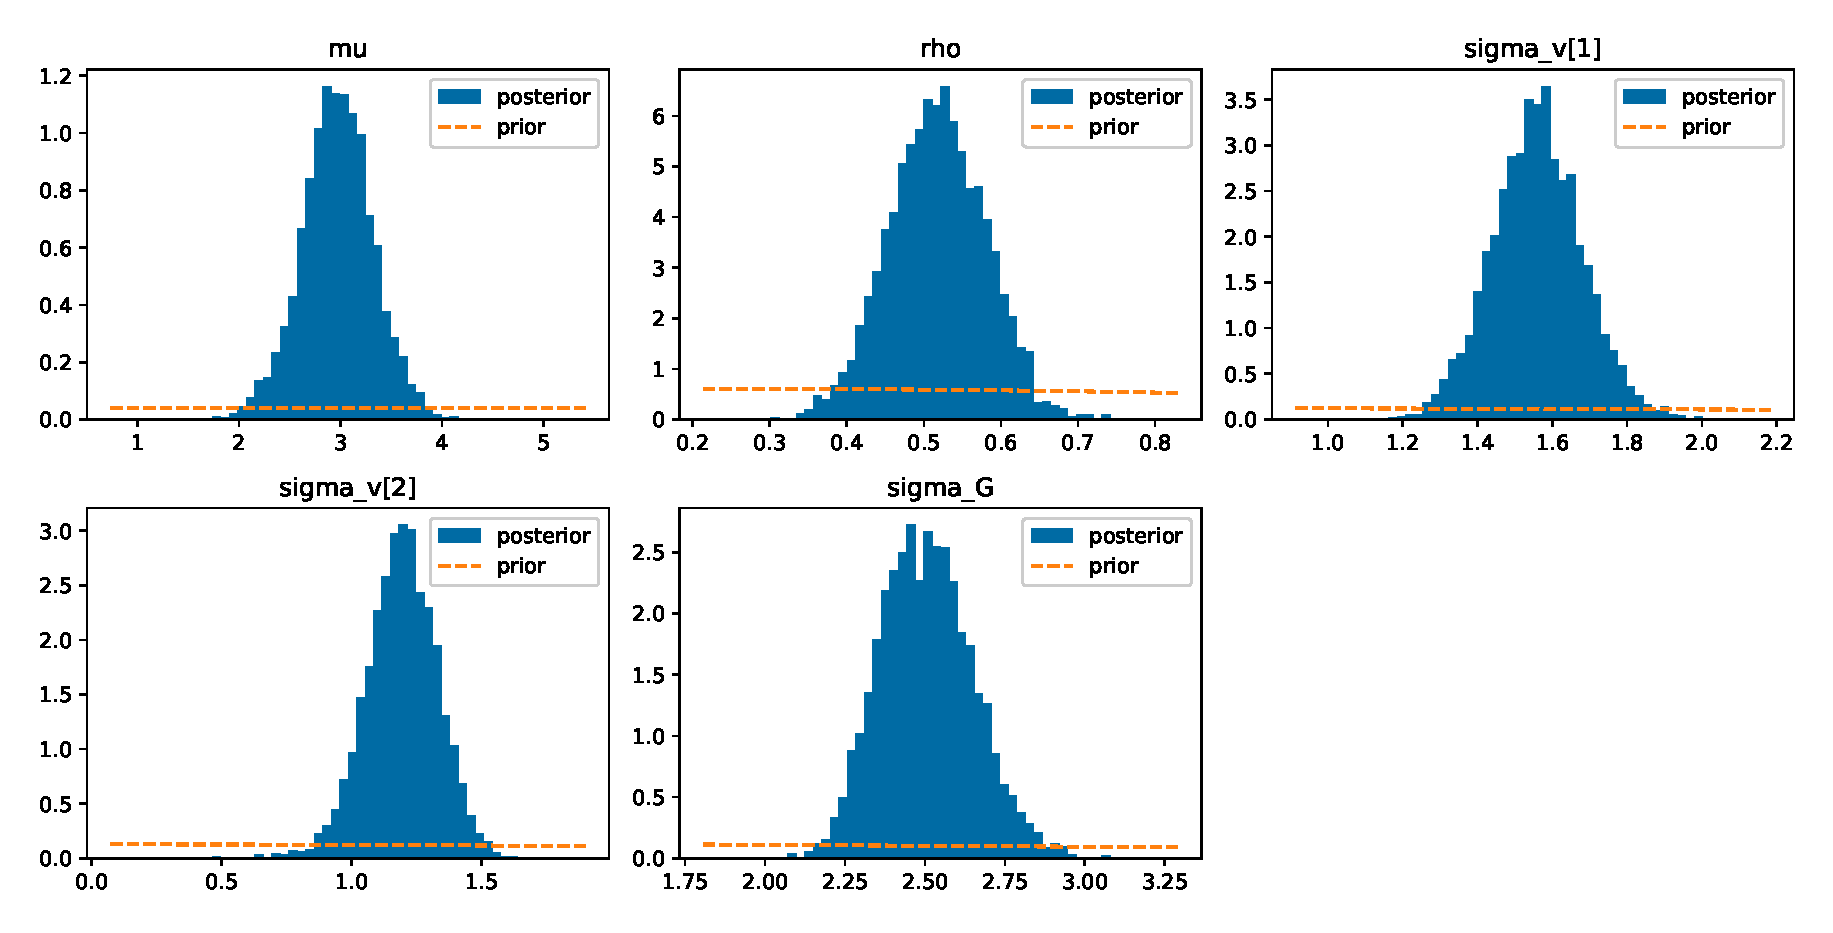
\includegraphics[width=\linewidth]{fig/factor_gdp_posterior_param.eps} \\
\bigskip
Note: \texttt{sigma\_v[1]} $= \sigma_E$, \texttt{sigma\_v[2]} $= \sigma_I$
\end{figure}
}

\frame{
\begin{figure}
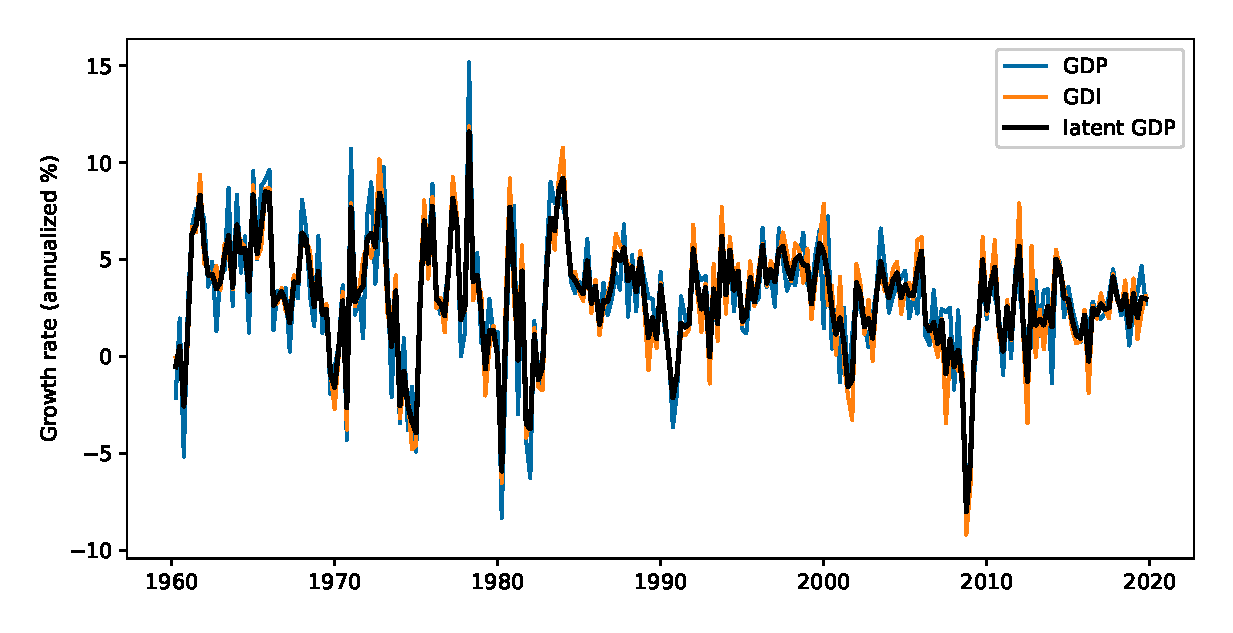
\includegraphics[width=\linewidth]{fig/factor_gdp_posterior_latent.eps} \\
\bigskip
Plot of $E[\tilde{s}_t \mid \bm{y}_1,\dots,\bm{y}_T]$ across $t$ \\[0.5\baselineskip]
Computed by averaging $\mu + \underbrace{E(s_t \mid \bm{y}_1,\dots,\bm{y}_T,\bm{\theta})}_\text{Kalman smoother}$ across parameter draws
\end{figure}
}

\frame{
\frametitle{What did we learn?}
\begin{itemize}
\item State space models
\begin{itemize}
\item Examples: dynamic factor model, ARMA
\end{itemize}
\item Kalman filter and smoother
\item Likelihood function $\Rightarrow$ Bayesian inference
\item Application: GDP measurement
\end{itemize}
}

\frame{
\frametitle{Looking ahead}
\begin{itemize}
\item Modeling time-varying parameters
\item Missing data
\item Mixed-frequency data
\item High-dimensional factor models
\item Models with regime switching
\end{itemize}
}

\end{document}